\documentclass[aspectratio=169, 10pt]{beamer}

\usetheme{Madrid}
\usecolortheme{whale}
\definecolor{mainblue}{RGB}{0,73,144}
\definecolor{accentred}{RGB}{180,30,40}
\definecolor{softgreen}{RGB}{34,139,34}
\definecolor{lightyellow}{RGB}{255,255,224}
\definecolor{lightgray}{RGB}{240,240,240}
\definecolor{oursgreen}{RGB}{232,245,233}
\setbeamercolor{structure}{fg=mainblue}
\setbeamercolor{alerted text}{fg=accentred}
\setbeamercolor{block title}{bg=mainblue, fg=white}
\setbeamercolor{block body}{bg=lightgray}
\setbeamertemplate{navigation symbols}{}
\setbeamertemplate{footline}[frame number]
\setlength{\parskip}{0pt}

\usepackage[utf8]{inputenc}
\usepackage[T1]{fontenc}
\usepackage{amsmath, amssymb, amsfonts}
\usepackage{booktabs}
\usepackage{graphicx}
\usepackage{tikz}
\usetikzlibrary{arrows.meta, positioning, shapes, calc, decorations.pathreplacing, fit}
\usepackage{multirow}
\usepackage{hyperref}
\usepackage{fontawesome5}
\usepackage{pifont}
\usepackage{colortbl}

\title[AI Code Detection]{%
  \textbf{Beyond Binary: Unified Detection and Attribution\\
  of AI-Generated Code via Hierarchical Family-Aware Learning}}
\subtitle{Research Proposal --- NeurIPS 2026}
\author{Student Name}
\institute{University Name}
\date{\today}

\begin{document}

\begin{frame}
\titlepage
\end{frame}

\begin{frame}{Outline}
\tableofcontents
\end{frame}


% ════════════════════════════════════════════════════════════════════════
\section{Problem: Why Binary Detection is Not Enough}
% ════════════════════════════════════════════════════════════════════════

\begin{frame}{Binary Detection is Solved --- The Real Challenges Remain}
\vspace{-0.2cm}
\begin{columns}[T]
\column{0.48\textwidth}
\begin{block}{Binary: Human vs Machine (CoDET-M4)}
\centering\footnotesize
\begin{tabular}{lc}
\toprule
\textbf{Method} & \textbf{F1 (\%)} \\
\midrule
SVM & 72.19 \\
CatBoost & 88.78 \\
CodeBERT & 95.70 \\
CodeT5 & 98.35 \\
UniXcoder & 98.65 \\
\rowcolor{oursgreen}
\textbf{SpectralCode (ours)} & \textbf{99.06} \\
\bottomrule
\end{tabular}
\end{block}
\vspace{0.05cm}
{\small \faExclamationTriangle\ $>$99\% F1 $\Rightarrow$ \alert{task is saturated}}

\column{0.50\textwidth}
\begin{alertblock}{Three Unsolved Challenges}
\small
\begin{enumerate}\setlength\itemsep{4pt}
    \item[\faUsers] \textbf{Authorship}: \emph{Which} LLM generated it? \\
    {\scriptsize (6--12 classes, best SOTA only 66\% F1)}
    \item[\faGlobeAmericas] \textbf{OOD}: Train Python $\to$ test Go? \\
    {\scriptsize (99\% $\to$ 30\% F1 collapse on AICD)}
    \item[\faShieldAlt] \textbf{Adversarial}: DPO-tuned mimicry? \\
    {\scriptsize (Models fine-tuned to write like humans)}
\end{enumerate}
\end{alertblock}
\end{columns}

\vspace{0.1cm}
\centering
\fbox{\parbox{0.85\textwidth}{\centering\small
\textbf{Our vision}: A unified method evaluated across \textbf{3 benchmarks}, \textbf{3.6M samples}, covering binary + attribution + OOD + adversarial}}
\end{frame}


\begin{frame}{The Bigger Picture: From Detection to Understanding}
\vspace{-0.1cm}

\begin{block}{The Evolution of the Threat}
\small
\begin{enumerate}\setlength\itemsep{4pt}
    \item[\textbf{2023}] ``Is this code written by AI?'' $\to$ Binary detection (\textbf{solved}: $>$99\% F1)
    \item[\textbf{2024}] ``Which model family generated it?'' $\to$ Attribution (\textbf{hard}: best 66\% F1, 6-class)
    \item[\textbf{2025}] ``Can the model fool the detector?'' $\to$ DPO-tuned adversarial code (DROID, EMNLP'25)
    \item[\textbf{2026}] ``Does it generalize to unseen languages?'' $\to$ OOD collapse: 99\% $\to$ 30\% (AICD, EACL'26)
\end{enumerate}
\end{block}

\vspace{0.1cm}
\begin{columns}[T]
\column{0.55\textwidth}
\begin{alertblock}{Why Current Methods Fail at Attribution}
\small
\begin{itemize}\setlength\itemsep{2pt}
    \item LLMs form \textbf{family trees}: Nxcode = fine-tuned Qwen1.5, CodeLlama = fine-tuned Llama
    \item Fine-tuned models inherit parent's ``stylometric DNA'' --- nearly identical coding patterns
    \item Standard classifiers treat all classes as \textbf{equidistant} $\to$ 40\%+ confusion between parent-child pairs
    \item Qwen1.5 F1 = 0.41 (near random for 6-class)
\end{itemize}
\end{alertblock}

\column{0.43\textwidth}
\begin{exampleblock}{\faLightbulb\ Our Key Insight}
\small
The family tree of LLMs is not a nuisance --- it is \textbf{structured prior knowledge}.\\[6pt]
Models within the same family should be \emph{closer but separable} in embedding space.\\[6pt]
\textbf{$\Rightarrow$ Encode genealogy as distance constraints}
\end{exampleblock}
\end{columns}
\end{frame}


% ════════════════════════════════════════════════════════════════════════
\section{Benchmarks: Three Complementary Challenges}
% ════════════════════════════════════════════════════════════════════════

\begin{frame}{Three Benchmarks --- Why These Three?}
\vspace{-0.25cm}
\begin{center}\footnotesize
\begin{tabular}{@{}lp{3.6cm}p{3.6cm}p{3.6cm}@{}}
\toprule
& \textbf{CoDET-M4} & \textbf{DroidCollection} & \textbf{AICDBench} \\
& {\tiny Orel et al., ACL Findings 2025} & {\tiny Orel et al., EMNLP 2025} & {\tiny Orel et al., EACL 2026} \\
\midrule
\textbf{Scale} & 500K samples & 1.06M samples & 2.05M samples \\
\textbf{Languages} & 3 (Py, Java, C++) & 7 languages & 9 languages \\
\textbf{Models} & 5 generators & 43 models, 11 families & 77 models, 11 families \\
\textbf{Sources} & CF, GitHub, LeetCode & General, Algo, Research & Algo, Research, General \\
\midrule
\textbf{Binary} & \ding{51} (saturated 99\%) & \ding{51} (saturated 97\%) & \ding{51} + \textbf{4-split OOD} \\
\textbf{Attribution} & \ding{51} 6-class & --- & \ding{51} 12-class family \\
\textbf{Refined} & \ding{55} & \ding{51} \textbf{3 scenarios} & \ding{51} (hybrid class) \\
\textbf{Adversarial} & \ding{55} & \ding{51} \textbf{DPO 157K pairs} & \ding{51} (in Task 3) \\
\bottomrule
\end{tabular}
\end{center}
\vspace{0.05cm}
\begin{columns}[T]
\column{0.32\textwidth}
\begin{exampleblock}{\scriptsize \faStar\ CoDET-M4: Attribution}
\scriptsize
Best for fine-grained authorship (6-class). Known Nxcode$\leftrightarrow$Qwen confusion. Per-lang/source breakdowns.
\end{exampleblock}

\column{0.32\textwidth}
\begin{exampleblock}{\scriptsize \faStar\ DROID: Adversarial}
\scriptsize
Machine-refined (continue, gap-fill, rewrite). DPO evasion attacks. Varied decoding strategies (temp, top-k, beam).
\end{exampleblock}

\column{0.32\textwidth}
\begin{exampleblock}{\scriptsize \faStar\ AICD: OOD Stress-Test}
\scriptsize
77 models incl.\ reasoning LLMs. Train 3 lang $\to$ test 9 lang. Progressive 4-split OOD evaluation.
\end{exampleblock}
\end{columns}
\end{frame}


% ════════════════════════════════════════════════════════════════════════
\section{Method 1: SpectralCode (Completed)}
% ════════════════════════════════════════════════════════════════════════

\begin{frame}{SpectralCode --- Architecture Pipeline}
\vspace{-0.2cm}
\begin{center}
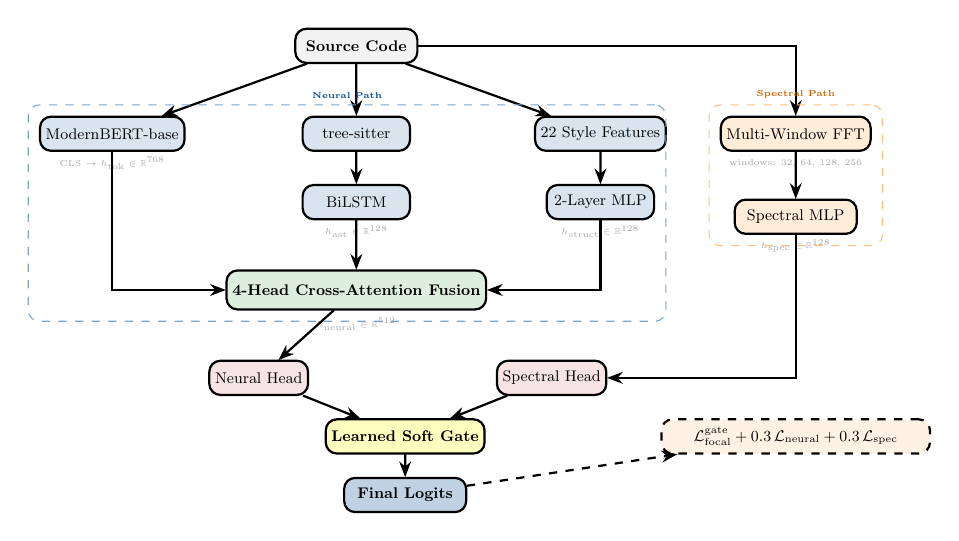
\begin{tikzpicture}[
    scale=0.62, transform shape,
    box/.style={draw, rounded corners, thick, font=\small, minimum height=0.7cm},
    enc/.style={box, fill=mainblue!15},
    proc/.style={box, fill=softgreen!15},
    head/.style={box, fill=accentred!12},
    arr/.style={-{Stealth[length=2mm]}, thick},
    dim/.style={font=\tiny, text=gray!70}
]
    % Input
    \node[box, fill=gray!10, minimum width=2.5cm] (code) at (0, 0) {\textbf{Source Code}};

    % Stream 1: Token
    \node[enc, minimum width=2.8cm] (bert) at (-5, -1.8) {ModernBERT-base};
    \node[dim] at (-5, -2.4) {CLS $\to h_{\text{tok}} \in \mathbb{R}^{768}$};

    % Stream 2: AST
    \node[enc, minimum width=2.2cm] (ts) at (0, -1.8) {tree-sitter};
    \node[enc, minimum width=2.2cm] (lstm) at (0, -3.2) {BiLSTM};
    \node[dim] at (0, -3.8) {$h_{\text{ast}} \in \mathbb{R}^{128}$};

    % Stream 3: Structural
    \node[enc, minimum width=2.2cm] (feat) at (5, -1.8) {22 Style Features};
    \node[enc, minimum width=2.2cm] (mlp1) at (5, -3.2) {2-Layer MLP};
    \node[dim] at (5, -3.8) {$h_{\text{struct}} \in \mathbb{R}^{128}$};

    \draw[arr] (code) -- (bert);
    \draw[arr] (code) -- (ts);
    \draw[arr] (ts) -- (lstm);
    \draw[arr] (code) -- (feat);
    \draw[arr] (feat) -- (mlp1);

    % Cross-Attention Fusion
    \node[proc, minimum width=5cm, minimum height=0.8cm] (xattn) at (0, -5) {\textbf{4-Head Cross-Attention Fusion}};
    \node[dim] at (0, -5.7) {$h_{\text{neural}} \in \mathbb{R}^{512}$};
    \draw[arr] (bert) |- (xattn);
    \draw[arr] (lstm) -- (xattn);
    \draw[arr] (mlp1) |- (xattn);

    % Stream 4: Spectral (separate path)
    \node[enc, fill=orange!15, minimum width=2.5cm] (fft) at (9, -1.8) {Multi-Window FFT};
    \node[dim] at (9, -2.4) {windows: 32, 64, 128, 256};
    \node[enc, fill=orange!15, minimum width=2.5cm] (smlp) at (9, -3.5) {Spectral MLP};
    \node[dim] at (9, -4.1) {$h_{\text{spec}} \in \mathbb{R}^{128}$};
    \draw[arr] (code) -| (fft);
    \draw[arr] (fft) -- (smlp);

    % Heads
    \node[head] (nh) at (-2, -6.8) {Neural Head};
    \node[head] (sh) at (4, -6.8) {Spectral Head};
    \draw[arr] (xattn) -- (nh);
    \draw[arr] (smlp) |- (sh);

    % Gate
    \node[proc, fill=yellow!25, minimum width=3cm] (gate) at (1, -8) {\textbf{Learned Soft Gate}};
    \draw[arr] (nh) -- (gate);
    \draw[arr] (sh) -- (gate);

    % Output
    \node[box, fill=mainblue!25, minimum width=2.5cm] (out) at (1, -9.2) {\textbf{Final Logits}};
    \draw[arr] (gate) -- (out);

    % Loss
    \node[box, fill=orange!10, dashed, minimum width=5.5cm] (loss) at (9, -8) {$\mathcal{L}_{\text{focal}}^{\text{gate}} + 0.3\,\mathcal{L}_{\text{neural}} + 0.3\,\mathcal{L}_{\text{spec}}$};
    \draw[arr, dashed] (out) -- (loss);

    % Annotations
    \node[draw, dashed, mainblue!50, rounded corners, fit=(bert)(lstm)(mlp1)(xattn), inner sep=4pt, label={[font=\tiny\bfseries, mainblue]above:Neural Path}] {};
    \node[draw, dashed, orange!50, rounded corners, fit=(fft)(smlp), inner sep=4pt, label={[font=\tiny\bfseries, orange!80!black]above:Spectral Path}] {};
\end{tikzpicture}
\end{center}
\end{frame}


\begin{frame}{SpectralCode --- What Makes Each Stream Novel?}
\vspace{-0.15cm}
\begin{columns}[T]
\column{0.32\textwidth}
\begin{block}{\faCode\ Neural Path}
\scriptsize
\textbf{Token}: ModernBERT-base (SDPA) \\
$\to$ CLS token, semantic+lexical \\[3pt]
\textbf{AST}: tree-sitter $\to$ 67 node types $\to$ BiLSTM \\
$\to$ syntactic structure \\[3pt]
\textbf{Structural}: 22 features --- indent patterns, naming style (snake\_case/camelCase ratio), comment density, complexity counts \\[3pt]
\textbf{Fusion}: 4-head cross-attention + gated projection $\to$ $h_{\text{neural}} \in \mathbb{R}^{512}$
\end{block}

\column{0.32\textwidth}
\begin{block}{\faWaveSquare\ Spectral Path (Novel)}
\scriptsize
\textbf{Key insight}: LLM decoding creates \emph{frequency artifacts} --- periodic patterns from autoregressive sampling (top-$k$, top-$p$, temperature). \\[3pt]
\textbf{Process}: \\
Token IDs $\to$ 1D signal $\to$ FFT at 4 windows (32, 64, 128, 256) \\[3pt]
\textbf{Per window} (16 features): \\
$\bullet$ 8 band energies \\
$\bullet$ Spectral centroid \\
$\bullet$ Rolloff, flatness, peak freq \\[3pt]
$\to$ 64-dim $\to$ MLP $\to$ $h_{\text{spec}} \in \mathbb{R}^{128}$\\[3pt]
{\tiny Inspired by deepfake spectral forensics (Frank et al., ICML 2020)}
\end{block}

\column{0.32\textwidth}
\begin{block}{\faBalanceScale\ Learned Gate}
\scriptsize
\textbf{Why?} Not all code benefits equally from spectral vs neural analysis. \\[3pt]
\textbf{Gate}: MLP([neural; spec]) $\to$ softmax weights $(w_n, w_s)$ \\[3pt]
$\text{logits} = w_n \cdot f_n(h_{\text{neural}}) + w_s \cdot f_s(h_{\text{spec}})$ \\[3pt]
\textbf{Auxiliary losses} on each head individually ensure both paths learn useful representations. \\[3pt]
\textbf{Total}: \\
$\mathcal{L}_{\text{focal}} + 0.3\,\mathcal{L}_{\text{neural}} + 0.3\,\mathcal{L}_{\text{spec}}$
\end{block}
\end{columns}
\end{frame}


% ════════════════════════════════════════════════════════════════════════
\section{Results: SpectralCode (Completed)}
% ════════════════════════════════════════════════════════════════════════

\begin{frame}{CoDET-M4: SpectralCode vs Paper Baselines (ACL Findings 2025)}
\vspace{-0.2cm}
\begin{columns}[T]
\column{0.48\textwidth}
\begin{block}{Binary Detection (Macro-F1 \%)}
\centering\footnotesize
\begin{tabular}{lcccc}
\toprule
& \textbf{P} & \textbf{R} & \textbf{F1} & \textbf{Acc} \\
\midrule
CatBoost & 88.7 & 88.8 & 88.8 & 88.8 \\
CodeBERT & 95.7 & 95.7 & 95.7 & 95.7 \\
CodeT5 & 98.4 & 98.4 & 98.4 & 98.4 \\
UniXcoder & 98.7 & 98.7 & 98.7 & 98.7 \\
\midrule
\rowcolor{oursgreen}
\textbf{Ours} & \textbf{99.1} & \textbf{99.1} & \textbf{99.1} & \textbf{99.1} \\
\bottomrule
\end{tabular}
\end{block}

\column{0.48\textwidth}
\begin{alertblock}{Author Attribution (6-class F1)}
\centering\footnotesize
\begin{tabular}{lc|c}
\toprule
& \textbf{F1} & $\boldsymbol{\Delta}$ \\
\midrule
SVM & 27.63 & --- \\
CatBoost & 45.42 & --- \\
CodeT5 & 62.45 & --- \\
CodeBERT & 64.80 & --- \\
UniXcoder & 66.33 & --- \\
\midrule
\rowcolor{oursgreen}
\textbf{SpectralCode} & \textbf{69.82} & \textcolor{softgreen}{+3.49} \\
\bottomrule
\end{tabular}
\end{alertblock}
\end{columns}

\vspace{0.1cm}
\begin{columns}[T]
\column{0.48\textwidth}
\begin{block}{Per-Language Author F1 (\%)}
\centering\footnotesize
\begin{tabular}{lccc}
\toprule
& \textbf{C++} & \textbf{Java} & \textbf{Python} \\
\midrule
SpectralCode & 72.31 & 70.12 & 69.22 \\
\bottomrule
\end{tabular}
\end{block}

\column{0.48\textwidth}
\begin{block}{Per-Source Author F1 (\%)}
\centering\footnotesize
\begin{tabular}{lccc}
\toprule
& \textbf{CF} & \textbf{GitHub} & \textbf{LC} \\
\midrule
SpectralCode & 77.17 & 56.18 & 60.35 \\
\bottomrule
\end{tabular}
{\tiny \alert{GitHub} is the main bottleneck ($\downarrow$21\% vs CF)}
\end{block}
\end{columns}
\end{frame}


\begin{frame}{DroidCollection: SpectralCode \textbf{Beats} DroidDetect-Base (EMNLP 2025)}
\vspace{-0.2cm}
\begin{columns}[T]
\column{0.55\textwidth}
\begin{block}{Comparison with DROID Paper (Weighted-F1 \%)}
\centering\footnotesize
\begin{tabular}{llcc}
\toprule
\textbf{Type} & \textbf{Method} & \textbf{3-cls} & \textbf{4-cls} \\
\midrule
\multirow{2}{*}{\textit{Zero-shot}} & Fast-DetectGPT & 64.54 & --- \\
& GPTZero & 49.10 & --- \\
\midrule
\multirow{2}{*}{\textit{Fine-tuned}} & CatBoost & 72.31 & --- \\
& GCN & 51.63 & --- \\
\midrule
\multirow{3}{*}{\textit{Full train}} & GPT-SnifferFT & 82.75 & --- \\
& CoDet-M4FT & 83.25 & --- \\
& DroidDetect-B & 86.76 & 92.95 \\
& DroidDetect-L & \textbf{88.78} & \textbf{94.30} \\
\midrule
\rowcolor{oursgreen}
\textit{Ours} & \textbf{SpectralCode} & \textbf{88.77} & \textbf{88.02} \\
\bottomrule
\end{tabular}

\vspace{2pt}
{\tiny All numbers: weighted-F1. DROID paper: domain-avg. Ours: overall.}
\end{block}

\column{0.43\textwidth}
\begin{exampleblock}{\faCheckCircle\ Key Findings}
\small
\begin{itemize}\setlength\itemsep{3pt}
    \item[\ding{51}] \textbf{Beats DroidDetect-Base} (88.77 $>$ 86.76)
    \item[\ding{51}] \textbf{Ties DroidDetect-Large} (88.77 $\approx$ 88.78)
    \item[\ding{51}] Beats \textbf{all} zero-shot \& fine-tuned
    \item[\faArrowRight] Using \textbf{base} model (149M) vs paper \textbf{large} (395M)!
\end{itemize}
\end{exampleblock}

\begin{alertblock}{\faStar\ Scaling Potential}
\small
Currently trained on only \textbf{100K / 1.06M} ($\sim$1/10) of DROID data.\\[3pt]
Full data training expected to improve further.
\end{alertblock}
\end{columns}
\end{frame}


\begin{frame}{AICDBench: Ongoing Exploration (EACL 2026)}
\vspace{-0.2cm}
\begin{columns}[T]
\column{0.55\textwidth}
\begin{block}{AICD Paper Baselines vs SpectralCode (Macro-F1 \%)}
\centering\footnotesize
\begin{tabular}{lccc}
\toprule
\textbf{Method} & \textbf{T1} {\tiny(2-cls)} & \textbf{T2} {\tiny(12-cls)} & \textbf{T3} {\tiny(4-cls)} \\
\midrule
CodeBERT & 28.64 & 23.71 & 55.60 \\
UniXcoder & 25.51 & 26.64 & 54.21 \\
DeBERTa & 34.13 & 12.08 & 54.65 \\
ModernBERT & \textbf{30.61} & \textbf{32.84} & \textbf{61.65} \\
\midrule
\rowcolor{oursgreen}
SpectralCode & 29.83 & 18.93 & 56.31 \\
\bottomrule
\end{tabular}

\vspace{3pt}
{\tiny Currently trained on \textbf{100K / 2.05M} ($\sim$1/20) of data}
\end{block}

\column{0.43\textwidth}
\begin{alertblock}{\faClock\ Status: Experimental}
\small
\begin{itemize}\setlength\itemsep{2pt}
    \item T1: Competitive with ModernBERT (29.83 vs 30.61)
    \item T3: Competitive (56.31 vs 61.65)
    \item T2: Below --- need family-aware loss
    \item[\faArrowRight] \textbf{Using only 1/20 of training data!}
\end{itemize}
\end{alertblock}

\begin{block}{\scriptsize \faExclamationTriangle\ AICD T1 OOD Collapse}
\scriptsize
Val 99.5\% $\to$ Test 29.8\% \textbf{across ALL methods}. 4-split progressive OOD (unseen langs + domains) is fundamentally hard.
\end{block}
\end{columns}
\end{frame}


% ════════════════════════════════════════════════════════════════════════
\section{Method 2: HierTreeCode (In Progress)}
% ════════════════════════════════════════════════════════════════════════

\begin{frame}{HierTreeCode --- SpectralCode + Hierarchical Affinity Loss}
\vspace{-0.15cm}
\begin{columns}[T]
\column{0.55\textwidth}
\begin{center}
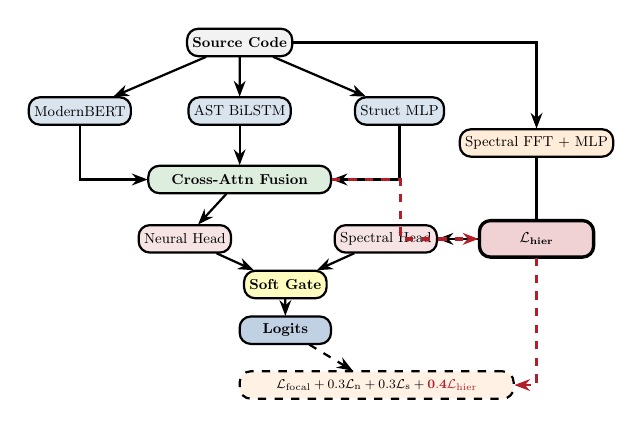
\begin{tikzpicture}[
    scale=0.58, transform shape,
    box/.style={draw, rounded corners, thick, font=\small, minimum height=0.6cm},
    enc/.style={box, fill=mainblue!15},
    proc/.style={box, fill=softgreen!15},
    head/.style={box, fill=accentred!12},
    arr/.style={-{Stealth[length=2mm]}, thick}
]
    \node[box, fill=gray!10, minimum width=2.2cm] (code) at (0, 0) {\textbf{Source Code}};

    \node[enc] (bert) at (-3.5, -1.5) {ModernBERT};
    \node[enc] (ast) at (0, -1.5) {AST BiLSTM};
    \node[enc] (struct) at (3.5, -1.5) {Struct MLP};
    \draw[arr] (code) -- (bert);
    \draw[arr] (code) -- (ast);
    \draw[arr] (code) -- (struct);

    \node[proc, minimum width=4cm] (xattn) at (0, -3) {\textbf{Cross-Attn Fusion}};
    \draw[arr] (bert) |- (xattn);
    \draw[arr] (ast) -- (xattn);
    \draw[arr] (struct) |- (xattn);

    \node[enc, fill=orange!15] (spec) at (6.5, -2.2) {Spectral FFT + MLP};
    \draw[arr] (code) -| (spec);

    \node[head] (nh) at (-1.2, -4.3) {Neural Head};
    \node[head] (sh) at (3.2, -4.3) {Spectral Head};
    \draw[arr] (xattn) -- (nh);
    \draw[arr] (spec) |- (sh);

    \node[proc, fill=yellow!25] (gate) at (1, -5.3) {\textbf{Soft Gate}};
    \draw[arr] (nh) -- (gate);
    \draw[arr] (sh) -- (gate);

    \node[box, fill=mainblue!25, minimum width=2cm] (out) at (1, -6.3) {\textbf{Logits}};
    \draw[arr] (gate) -- (out);

    % Hier loss branch (right side, clean)
    \node[box, fill=accentred!20, very thick, minimum width=2.5cm, minimum height=0.8cm] (hier) at (6.5, -4.3) {\textbf{$\mathcal{L}_{\text{hier}}$}};
    \draw[arr, accentred, very thick, dashed] (xattn.east) -- ++(1.5,0) |- (hier);

    % Loss
    \node[box, fill=orange!10, dashed, minimum width=6cm, font=\footnotesize] (loss) at (3, -7.5) {$\mathcal{L}_{\text{focal}} + 0.3\mathcal{L}_{\text{n}} + 0.3\mathcal{L}_{\text{s}} + \textcolor{accentred}{\mathbf{0.4\mathcal{L}_{\text{hier}}}}$};
    \draw[arr, dashed] (out) -- (loss);
    \draw[arr, accentred, dashed] (hier) |- (loss);
\end{tikzpicture}
\end{center}

\column{0.43\textwidth}
\begin{alertblock}{\faStar\ Hierarchical Affinity Loss}
\scriptsize
\textbf{Family Tree} (adapts per benchmark):\\[2pt]
\begin{tabular}{ll}
Qwen & $\to$ \{Qwen1.5, Nxcode\} \\
Meta & $\to$ \{Llama3.1, CodeLlama\} \\
Google & $\to$ \{Gemma, Gemini\} \\
\end{tabular}\\[4pt]
\textbf{Batch-hard triplet}:
$$[\,d_{\text{pos}}^{\max} - d_{\text{neg}}^{\min} + \alpha\,]_+$$
$d$: cosine distance on $\ell_2$-norm $h_{\text{neural}}$\\
$\alpha = 0.3$ margin\\[4pt]
\textbf{Effect}: Forces same-family closer, different-family further apart.
\end{alertblock}

\begin{block}{\scriptsize Difference from SpectralCode}
\scriptsize
SpectralCode = this diagram \textbf{without} the red $\mathcal{L}_{\text{hier}}$ branch. Everything else is identical.
\end{block}
\end{columns}
\end{frame}


\begin{frame}{HierTreeCode: Preliminary Results + Expected Impact}
\vspace{-0.15cm}
\begin{columns}[T]
\column{0.48\textwidth}
\begin{block}{CoDET-M4 Author F1 (\ding{51} Done)}
\centering\footnotesize
\begin{tabular}{lcc}
\toprule
& \textbf{Author F1} & $\boldsymbol{\Delta}$ vs UniX \\
\midrule
UniXcoder & 66.33 & --- \\
SpectralCode & 69.82 & +3.49 \\
\rowcolor{oursgreen}
\textbf{HierTreeCode} & \textbf{70.55} & \textbf{+4.22} \\
\bottomrule
\end{tabular}

\vspace{0.1cm}
{\scriptsize Per-generator F1 (HierTreeCode):}
\scriptsize
\begin{tabular}{lccc}
\toprule
Human & GPT & Llama & CodeLlama \\
\midrule
0.87 & 0.92 & 0.67 & 0.74 \\
\bottomrule
\end{tabular}
\begin{tabular}{lcc}
\toprule
\alert{Qwen1.5} & \alert{Nxcode} & Macro \\
\midrule
\textbf{0.44} {\tiny(+.03)} & \textbf{0.59} & \textbf{70.55} \\
\bottomrule
\end{tabular}
\end{block}

\column{0.50\textwidth}
\begin{alertblock}{\faStar\ Why HierTreeCode Will Help Further}
\small
\begin{itemize}\setlength\itemsep{3pt}
    \item \textbf{DROID T3/T4}: Family hierarchy (human $\to$ refined $\to$ machine $\to$ adversarial)
    \item \textbf{AICD T2} (12-class): Groups Google (Gemma+Gemini), Chinese AI (DeepSeek+Qwen)
    \item \textbf{AICD T3}: Adversarial $\approx$ machine origin
    \item Family tree adapts per benchmark automatically
\end{itemize}
\end{alertblock}

\begin{exampleblock}{\scriptsize Hierarchical Affinity Loss}
\scriptsize
$\mathcal{L}_{\text{hier}} = \frac{1}{|\mathcal{A}|}\sum_{i}[d_{i,p^*} - d_{i,n^*} + \alpha]_+$\\[2pt]
$p^*$: farthest same-family (hard positive)\\
$n^*$: closest diff-family (hard negative)\\
Cosine distance on $\ell_2$-normalized $h_{\text{neural}}$
\end{exampleblock}
\end{columns}
\end{frame}


% ════════════════════════════════════════════════════════════════════════
\section{Evaluation Plan \& Timeline}
% ════════════════════════════════════════════════════════════════════════

\begin{frame}{Full Evaluation Matrix}
\vspace{-0.2cm}
\begin{center}\footnotesize
\renewcommand{\arraystretch}{1.05}
\begin{tabular}{@{}p{2.5cm}p{3cm}p{3cm}p{3.2cm}@{}}
\toprule
& \textbf{CoDET-M4} {\tiny ACL'25} & \textbf{DROID} {\tiny EMNLP'25} & \textbf{AICD} {\tiny EACL'26} \\
\midrule
\textbf{Binary} & \textcolor{softgreen}{\ding{51}} 99.06\% & \textcolor{softgreen}{\ding{51}} 88.77\%$^w$ T3 & \textcolor{orange}{\faClock} 29.83\% T1 \\
\textbf{Attribution} & \textcolor{softgreen}{\ding{51}} 70.55\% (6-cls) & --- & \textcolor{orange}{\faClock} T2 (12-cls) \\
\textbf{Refined} & --- & \textcolor{softgreen}{\ding{51}} 88.77\%$^w$ T3 & \textcolor{orange}{\faClock} T3 \\
\textbf{Adversarial} & --- & \textcolor{softgreen}{\ding{51}} 88.02\%$^w$ T4 & \textcolor{orange}{\faClock} T3 \\
\textbf{OOD Lang} & \textcolor{orange}{\faClock} LOO & --- & \textcolor{orange}{\faClock} 3$\to$9 lang \\
\bottomrule
\end{tabular}
\end{center}

\vspace{0.05cm}
\begin{center}
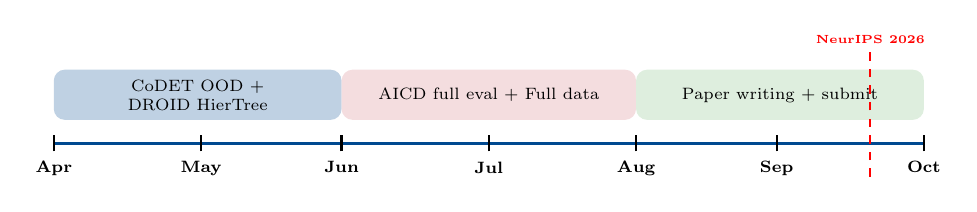
\begin{tikzpicture}[scale=0.85, transform shape]
    \draw[very thick, mainblue] (0, 0) -- (13, 0);
    \foreach \x/\m in {0/Apr, 2.2/May, 4.3/Jun, 6.5/Jul, 8.7/Aug, 10.8/Sep, 13/Oct} {
        \draw[thick] (\x, -0.12) -- (\x, 0.12);
        \node[below, font=\scriptsize\bfseries] at (\x, -0.15) {\m};
    }
    \fill[mainblue!25, rounded corners] (0, 0.35) rectangle (4.3, 1.1);
    \node[font=\scriptsize, text width=3.5cm, align=center] at (2.15, 0.72) {CoDET OOD + DROID HierTree};
    \fill[accentred!15, rounded corners] (4.3, 0.35) rectangle (8.7, 1.1);
    \node[font=\scriptsize, text width=3.5cm, align=center] at (6.5, 0.72) {AICD full eval + Full data};
    \fill[softgreen!15, rounded corners] (8.7, 0.35) rectangle (13, 1.1);
    \node[font=\scriptsize, text width=3.5cm, align=center] at (10.85, 0.72) {Paper writing + submit};
    \draw[dashed, red, thick] (12.2, -0.5) -- (12.2, 1.4);
    \node[font=\tiny\bfseries, text=red] at (12.2, 1.55) {NeurIPS 2026};
\end{tikzpicture}
\end{center}
\end{frame}


\begin{frame}{Contributions \& Summary}
\vspace{-0.1cm}
\begin{exampleblock}{Technical Contributions}
\small
\begin{enumerate}\setlength\itemsep{2pt}
    \item \textbf{SpectralCode}: Multi-stream (token + AST + structural + spectral FFT) with cross-attention + gating --- \emph{SOTA on CoDET-M4, beats DroidDetect-Base on DROID}
    \item \textbf{HierTreeCode}: First use of LLM genealogy as structured prior --- encodes parent-child as embedding distance constraints via batch-hard triplet mining
    \item \textbf{Unified 3-benchmark evaluation}: First work covering CoDET-M4 + DROID + AICD --- binary + attribution + OOD + adversarial in one method
    \item \textbf{Scaling insight}: Competitive results using only 1/10--1/20 of training data --- full data expected to close remaining gaps
\end{enumerate}
\end{exampleblock}

\begin{block}{Results So Far}
\centering\footnotesize
\begin{tabular}{lccc}
\toprule
& \textbf{CoDET-M4} & \textbf{DROID} & \textbf{AICD} \\
\midrule
Binary & 99.06\% (\textcolor{softgreen}{+0.41 vs UniX}) & 88.77\%$^w$ (\textcolor{softgreen}{$>$DroidDet-B}) & \faClock\ ongoing \\
Author & 70.55\% (\textcolor{softgreen}{+4.22 vs UniX}) & --- & \faClock\ T2 \\
Data used & 100K/500K & \alert{100K/1.06M} & \alert{100K/2.05M} \\
\bottomrule
\end{tabular}
\end{block}
\end{frame}


% ════════════════════════════════════════════════════════════════════════
\section{Experiment Insights}
% ════════════════════════════════════════════════════════════════════════

\begin{frame}{CoDET-M4: 10 Methods Explored --- What Worked and What Didn't}
\vspace{-0.2cm}
\begin{columns}[T]
\column{0.55\textwidth}
\begin{block}{Full Leaderboard (Author 6-class F1)}
\centering\scriptsize
\begin{tabular}{clcc}
\toprule
\textbf{\#} & \textbf{Method} & \textbf{Author F1} & \textbf{Key Idea} \\
\midrule
\rowcolor{oursgreen}
1 & \textbf{HierTreeCode} & \textbf{70.55} & Family tree loss \\
2 & RAGDetect & 70.46 & Retrieval-augmented \\
3 & BiScopeCode & 70.20 & MLM memorization \\
4 & TTACode & 70.20 & Test-time adapt \\
5 & MultiGranCode & 70.19 & CharCNN fusion \\
6 & GroupDRO & 70.17 & Worst-group opt \\
7 & SelfDistillCode & 70.14 & EMA distillation \\
8 & ProtoCon & 70.13 & Prototype + unif \\
\rowcolor{oursgreen}
9 & SpectralCode & 69.82 & FFT spectral \\
10 & GraphStyleCode & 69.71 & GAT on AST \\
\midrule
\textcolor{red}{---} & \textcolor{red}{EAGLECode} & \textcolor{red}{62.89} & \textcolor{red}{DANN (failed)} \\
\bottomrule
\end{tabular}
\end{block}

\column{0.43\textwidth}
\begin{alertblock}{\faExclamationTriangle\ DANN Catastrophically Fails}
\scriptsize
Gradient reversal forces generator-invariant features --- this \emph{directly opposes} attribution.\\
Qwen1.5 F1 drops to \textbf{0.198} (random).\\
\textbf{Lesson}: Domain adversarial $\neq$ attribution.
\end{alertblock}

\begin{exampleblock}{\faLightbulb\ Key Insights}
\scriptsize
\begin{itemize}\setlength\itemsep{1pt}
    \item All methods cluster in 69.7--70.6\% author F1
    \item Qwen1.5/Nxcode confusion is THE bottleneck
    \item GitHub source $\downarrow$21\% vs CodeForces
    \item GAT on AST provides no benefit
    \item Spectral FFT is surprisingly effective
\end{itemize}
\end{exampleblock}
\end{columns}
\end{frame}


\begin{frame}{AICD + DROID: 13 Deep Methods --- Cross-Benchmark Insights}
\vspace{-0.2cm}
\begin{columns}[T]
\column{0.50\textwidth}
\begin{block}{Leaderboard (5 completed methods)}
\centering\scriptsize
\begin{tabular}{clccc}
\toprule
\textbf{\#} & \textbf{Method} & \textbf{AICD} & \textbf{DROID} & \textbf{Avg} \\
\midrule
\rowcolor{oursgreen}
1 & SpectralCode & .350 & .847 & \textbf{.549} \\
2 & TokenStat & .330 & \textbf{.852} & .539 \\
3 & MoE-Code & .324 & .849 & .534 \\
4 & SlotCode & .329 & .839 & .533 \\
5 & DomainMix & .286 & .716 & .458 \\
\bottomrule
\end{tabular}
\end{block}

\begin{alertblock}{\scriptsize Methods That Failed}
\scriptsize
\textbf{CausAST}: Ortho $\to$ 0 (worst) | \textbf{OSCP}: Whitening dominates | \textbf{AST-IRM}: Penalty explodes to 5000
\end{alertblock}

\column{0.48\textwidth}
\begin{exampleblock}{\faLightbulb\ Cross-Benchmark Insights}
\small
\begin{enumerate}\setlength\itemsep{3pt}
    \item \textbf{AICD T1 OOD unsolved}: Val 99.5\% $\to$ Test 30\% for ALL methods
    \item \textbf{Spectral features transfer best}: Wins overall despite simplicity
    \item \textbf{Token stats are powerful}: Entropy, burstiness, Yule-K beat complex architectures on DROID
    \item \textbf{Mixup helps OOD}: DomainMix achieves best AICD T1 via embedding mixup
    \item \textbf{Only 1/10--1/20 data used}: Full data $\to$ higher scores expected
\end{enumerate}
\end{exampleblock}
\end{columns}
\end{frame}


\begin{frame}{}
\vspace{1.5cm}
\begin{center}
{\Huge \textbf{Thank You}}
\vspace{0.8cm}

{\Large Questions \& Discussion}
\vspace{1cm}

{\small
\faDatabase\ CoDET-M4 {\tiny(ACL Findings'25)} $\cdot$ DroidCollection {\tiny(EMNLP'25)} $\cdot$ AICDBench {\tiny(EACL'26)} \\[4pt]
\faGithub\ Code and experiments available upon request
}
\end{center}
\end{frame}

\end{document}
